%\documentclass[sigconf,timestamp]{acmart}
\documentclass[nonacm=true,acmlarge]{acmart}
\fancyhead{}

\usepackage{booktabs} % For formal tables

% Copyright
\setcopyright{none}
%\setcopyright{acmcopyright}
%\setcopyright{acmlicensed}
%\setcopyright{rightsretained}
%\setcopyright{usgov}
%\setcopyright{usgovmixed}
%\setcopyright{cagov}
%\setcopyright{cagovmixed}


% DOI
%\acmDOI{10.475/123_4}

% ISBN
%\acmISBN{123-4567-24-567/08/06}

%Conference
%\acmConference[CPS-SPC'18]{ACM Workshop on Cyber-Physical Systems Security \& Privacy}{October 2018}{Toronto, Canada}
%\acmYear{2018}
%\copyrightyear{2018}

% These commands are optional
%\acmBooktitle{Transactions of the ACM Woodstock conference}
%\editor{Jennifer B. Sartor}
%\editor{Theo D'Hondt}
%\editor{Wolfgang De Meuter}

%%% Custom packages
%
%\usepackage{subcaption} % recommended by ACM for subfigures
\usepackage[caption=false,font=small]{subfig}

\usepackage{pgfplots}
\pgfplotsset{width=10cm,compat=1.9}
\usepgfplotslibrary{fillbetween}

%
%\usepackage{pgf-umlsd}
%\usetikzlibrary{shadows,positioning}

\usetikzlibrary{arrows,shadows,positioning}


%%% Custom commands
%
\newcommand{\todo}[1]{\marginpar{\bf\large$[\ast]$}{\sf [#1]}}

\usepackage{k}
\lstset{language=k}

\newcommand{\langl}{\begin{picture}(4.5,7)
\put(1.1,2.5){\rotatebox{60}{\line(1,0){5.5}}}
\put(1.1,2.5){\rotatebox{300}{\line(1,0){5.5}}}
\end{picture}}
\newcommand{\rangl}{\begin{picture}(4.5,7)
\put(.9,2.5){\rotatebox{120}{\line(1,0){5.5}}}
\put(.9,2.5){\rotatebox{240}{\line(1,0){5.5}}}
\end{picture}}

\begin{document}
\title[The Beacon Chain in K]
{An Executable K Model of Ethereum 2.0 Beacon Chain Phase 0 Specification}
%\titlenote{Produces the permission block, and
%  copyright information}
%\subtitle{Extended Abstract}
%\subtitlenote{The full version of the author's guide is available as
%  \texttt{acmart.pdf} document}

%%%
\author{Denis Bogdanas}
%\author{ }
%\authornote{Dr.~Trovato insisted his name be first.}
\affiliation{%
  \institution{Runtime Verification Inc.}
%  \streetaddress{P.O. Box 840}
%  \city{Dhahran, Saudi Arabia}
%  \state{Ohio}
}
\email{denis.bogdanas@runtimeverification.com}

%%%
\author{Daejun Park}
%\author{ }
%\authornote{Dr.~Trovato insisted his name be first.}
\affiliation{%
  \institution{Runtime Verification Inc.}
%  \streetaddress{P.O. Box 840}
%  \city{Dhahran, Saudi Arabia}
%  \state{Ohio}
}
\email{daejun.park@runtimeverification.com}

%%%
\author{Chris Hathhorn}
%\author{ }
%\authornote{Dr.~Trovato insisted his name be first.}
\affiliation{%
  \institution{Runtime Verification Inc.}
%  \streetaddress{P.O. Box 840}
%  \city{Dhahran, Saudi Arabia}
%  \state{Ohio}
}
\email{chris.hathhorn@runtimeverification.com}

\author{Musab A. Alturki}
%\author{ }
%\authornote{Dr.~Trovato insisted his name be first.}
\orcid{0001-7957-1081}
\affiliation{%
  \institution{Runtime Verification Inc.}
%  \streetaddress{P.O. Box 840}
%  \city{Dhahran, Saudi Arabia}
%  \state{Ohio}
}
\email{musab.alturki@runtimeverification.com}

\author{Grigore Ro\c su}
%\author{ }
%\authornote{Dr.~Trovato insisted his name be first.}
%\orcid{0001-7957-1081}
\affiliation{%
  \institution{Runtime Verification, Inc.}
%  \streetaddress{P.O. Box 840}
%  \city{Dhahran, Saudi Arabia}
%  \state{Ohio}
}
\affiliation{%
%  \department{Information and Computer Science Department}
  \institution{University of Illinois at Urbana-Champaign}
%  \streetaddress{P.O. Box 840}
%  \city{Dhahran, Saudi Arabia}
%  \state{Ohio}
%  \postcode{34464-8044}
}
\email{grosu@illinois.edu}

% The default list of authors is too long for headers.
\renewcommand{\shortauthors}{Alturki and Ro\c su}


\begin{abstract}
This report describes an executable formal model in the K framework of Ethereum's Beacon Chain Phase
0 specification. We highlight the structure of the model, explain how the beacon chain state
transition and the supporting functions are specified and then outline how the model can be
validated using the standard beacon chain test suite. We present general test coverage analysis and
a summary of our findings and recommendations. The full specification is available online at
\url{https://github.com/runtimeverification/beacon-chain-spec}.
\end{abstract}


%\copyrightyear{2018}
%\acmYear{2018}
%\setcopyright{acmcopyright}
%\acmConference[CPS-SPC '18]{2018 Workshop on Cyber-Physical Systems Security and PrivaCy}{October 19, 2018}{Toronto, ON, Canada}
%\acmBooktitle{CPS-SPC '18: 2018 Workshop on Cyber-Physical Systems Security and PrivaCy Oct. 19, 2018, Toronto, ON, Canada}
%\acmPrice{15.00}
%\acmDOI{10.1145/3264888.3264895}
%\acmISBN{978-1-4503-5992-4/18/10}

%\CopyrightYear{2018}
%\setcopyright{acmcopyright}
%\conferenceinfo{CPS-SPC '18,}{October 19, 2018, Toronto, ON, Canada}
%\isbn{978-1-4503-5992-4/18/10}\acmPrice{$15.00}
%\doi{https://imsva91-ctp.trendmicro.com:443/wis/clicktime/v1/query?url=https%3a%2f%2fdoi.org%2f10.1145%2f3264888.3264895&umid=1272F148-7316-1905-A8B2-21A2B8EE9BE6&auth=ec34f7633709e8bd85e48c7fc0c92c09c079e558-4b58fbd6a20241a010ea046d5792f330788363a7}

%
% The code below should be generated by the tool at
% http://dl.acm.org/ccs.cfm
% Please copy and paste the code instead of the example below.
%
%\begin{CCSXML}
%<ccs2012>
%<concept>
%<concept_id>10002978.10002986</concept_id>
%<concept_desc>Security and privacy~Formal methods and theory of security</concept_desc>
%<concept_significance>500</concept_significance>
%</concept>
%<concept>
%<concept_id>10002978.10002986.10002990</concept_id>
%<concept_desc>Security and privacy~Logic and verification</concept_desc>
%<concept_significance>500</concept_significance>
%</concept>
%<concept>
%<concept_id>10002978.10002991.10002993</concept_id>
%<concept_desc>Security and privacy~Access control</concept_desc>
%<concept_significance>500</concept_significance>
%</concept>
%<concept>
%<concept_id>10010520.10010553</concept_id>
%<concept_desc>Computer systems organization~Embedded and cyber-physical systems</concept_desc>
%<concept_significance>500</concept_significance>
%</concept>
%<concept>
%<concept_id>10011007.10010940.10010992.10010998.10003791</concept_id>
%<concept_desc>Software and its engineering~Model checking</concept_desc>
%<concept_significance>500</concept_significance>
%</concept>
%</ccs2012>
%\end{CCSXML}
%
%\ccsdesc[500]{Security and privacy~Formal methods and theory of security}
%\ccsdesc[500]{Security and privacy~Logic and verification}
%\ccsdesc[500]{Security and privacy~Access control}
%\ccsdesc[500]{Computer systems organization~Embedded and cyber-physical systems}
%\ccsdesc[500]{Software and its engineering~Model checking}
%
%\keywords{Distance-bounding protocols, Distance fraud, Probabilistic rewriting, Statistical model checking, {\sc Maude}}
%
\settopmatter{printfolios=true}  %%% show page numbers
\maketitle

\section{Introduction}

Consensus in Ethereum has so far been based on a proof-of-work protocol. However, due to
computational efficiency and energy consumption considerations, Ethereum is undergoing a transition
into a proof-of-stake-based consensus protocol, namely Casper, in which the choice of the next
block-proposing validator node is proportional to its share at stake in the network (rather than its
hash power). Casper’s design aims at guaranteeing desirable safety and liveness properties of
transaction blocks. Furthermore, to significantly increase transaction throughput and address
scalability concerns, Sharding has also been proposed as another major update to Ethereum. A shard
is a partition of a larger blockchain system that maintains its own state and transaction history.
Both Casper and Sharding, along with several other planned major updates, will be part of a major
future version of Ethereum, called Ethereum 2.0 (a.k.a. Serenity). To facilitate a smooth
transition, development is planned to take place in seven phases. The first phase, Phase 0, targets
fully specifying the main PoS chain in Ethereum 2.0, called the beacon chain, which maintains
validator records and manages validator attestations, in addition to laying the foundation for a
specification of shards.

As our ultimate goal is to have a formal framework for specifying, executing and verifying Casper
and Sharding, we introduce in this report a first-step towards achieving this goal, which is an
executable, formal specification of the full beacon chain specification given by "Ethereum 2.0 Phase
0" in the K framework. The specification is formal, defining node states as configuration patterns
and specifying protocol operations and behaviors as transitions over patterns, modeled as rewrite
rules. Furthermore, the specification is executable by pattern rewriting in the K tool, which
provides immediately (at no extra cost) an execution engine for the protocol.

Executable specifications not only enable running simulations and animating systems, which can be a
tremendously useful tool for prototyping and debugging different designs during the development
process, but can also be used as reference implementations for model-based test generation and for
validating other implementations. Perhaps more importantly, the specification itself can be used
(through K’s recently developed LLVM backend) to deploy a correct-by-construction implementation
that is reasonably efficiently executable.   Furthermore, such an approach will seamlessly enable
further refining the protocol’s formal design without having to worry about modifying the
implementation. Finally, the executable specification of the protocol in K is immediately available
to K’s (ever-expanding) arsenal of reachability, model checking and theorem proving tools,
facilitating various forms of formal analysis of properties.

In addition, we aim for this Phase 0 specification to lay the foundation for both: (1) further
future extensions corresponding to new features or components that may appear in later phases of
development of Ethereum 2.0, and (2) further formal modeling and verification developments.

The full specification developed in this work is available online at
\url{https://github.com/runtimeverification/beacon-chain-spec}.  %and at
\url{https://github.com/runtimeverification/rdao-smc-minimal}. Both repositories  The repository
includes documented specifications, compilation instructions and scripts for running the tests
described in this report.

The rest of the report is organized as follows. In Section~\ref{sec:bc} below, we give an overview
of the beacon chain. This is followed in Section~\ref{sec:bck} by a description of our model of the
beacon chain in K. In Section~\ref{sec:testing} we outline how the model is validated against
existing tests. Section~\ref{sec:coverage} describes test coverage analysis, along with findings and
recommendations. The report concludes in Section~\ref{sec:conc} with a discussion of possible future
developments.

\section{Ethereum 2.0 Beacon Chain Phase 0}
\label{sec:bc}

The beacon chain is the main chain of the proof-of-stake protocol layer of the upcoming Ethereum
2.0. The chain consists of a sequence of beacon blocks containing information pertaining to various
aspects of the protocol, including validators and deposits, attestations and committees,
justification and finalization, rewards and penalties, shards and crosslinks, and hashing and
merkleization, in addition to the state of the underlying proof-of-work Ethereum 1.0 blockchain. The
reference specification of the beacon chain protocol that maintains this chain is given by its
implementation in Python, available at
\url{https://github.com/ethereum/eth2.0-specs/blob/dev/specs/core/0_beacon-chain.md}.

The protocol progresses temporally with respect to a logical timeline in which time is divided into
epochs, which are further divided into a fixed number of individual short periods of time called
slots. Figure~\ref{fig:eth2timeline} (borrowed from
\url{https://github.com/protolambda/eth2-docs/blob/master/README.md}) illustrates this timeline.

\begin{figure}[h]
\centering
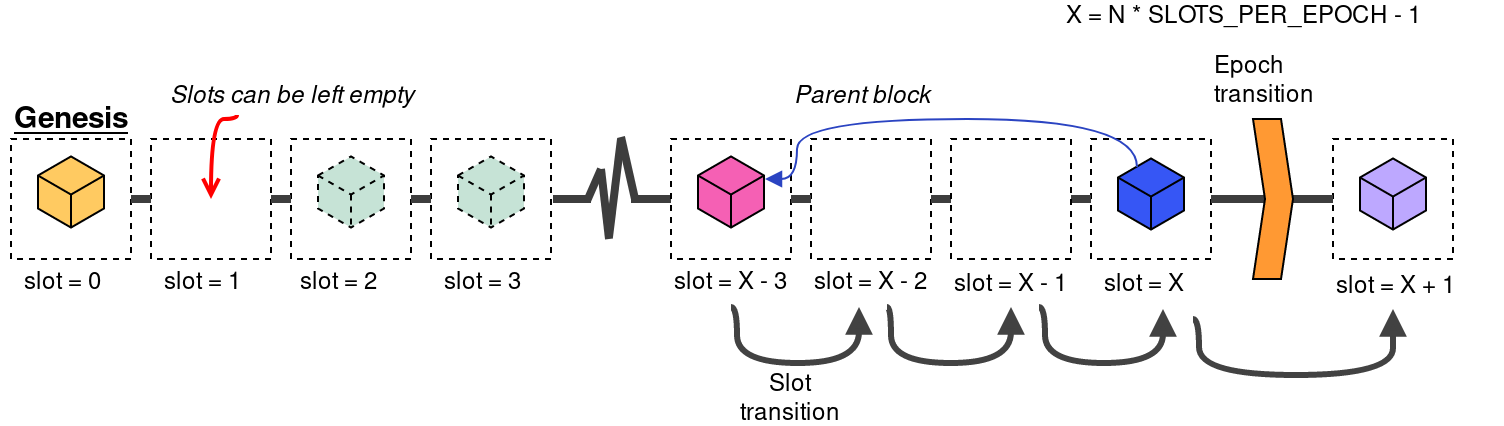
\includegraphics[width=\textwidth]{assets/eth2-timeline.png}
\caption{An illustration of Eth 2.0 timeline (\url{https://github.com/protolambda/eth2-docs/blob/master/README.md})}
\label{fig:eth2timeline}
\end{figure}

During each slot, a designated validator (called a proposer) from a committee selected through a
RANDAO-like shuffling process proposes a new beacon chain block, and all other validators in that
committee submit their attestations (for this and possibly other blocks floating around). An
attestation is a vote for a block. Attestations serve several different purposes in the protocol and
are at the heart of its operation. For example, an attestation confirms progression to the block's
slot, identifies the block's parent in the chain (fork choice rule), contributes to deciding
finality of blocks (Casper FFG) and links to the block's shard in case the block does not belong to
the main chain (crosslinks).

An epoch transition takes place when progressing across epoch-boundary slots. Much of the protocol
processing happens during an epoch transition. Examples include: processing justification and
finalization of blocks according to Casper, updating crosslinks, rewarding well-behaving validators
and penalizing ones that deviated from the protocol, and processing deposits to join in as
validators and requests to withdraw deposits and exit from the system.

Two core components of the specification of the beacon chain are: (1) the beacon chain state and (2)
the beacon chain state transition function. The beacon chain state maintains information about the
chain itself (where it currently fits within a view of the network), the current time slot, a full
registry of validators and their states, all pending attestations, crosslinks to shards, finality
information, a link to the underlying Ethereum 1.0 blockchain, among other things. The state
includes all pieces of information needed for the proper functioning of the protocol.

The state is processed by the second core component of the specification, which is the beacon chain
state transition function.  Given the next beacon block to be processed, the function transforms a
given beacon chain state (pre-state) into a new state (post-state) that reflects the results of
progressing time up to the block's slot value (and performing epoch-transition processing if
appropriate) and then processing the block's contents. An excerpt of the relevant part of the
function's specification in Python is shown below:
\begin{lstlisting}[language=python, basicstyle=\small, tabsize=2, columns=flexible,
               basicstyle=\ttfamily]
def state_transition(state: BeaconState, block: BeaconBlock ...) -> BeaconState:
  # Process slots (including those with no blocks) since block
  process_slots(state, block.slot)
  # Process block
  process_block(state, block)
  ...
  # Return post-state
  return state
\end{lstlisting}

Processing begins at the genesis state (the state having the genesis beacon block already
processed). When processing a (non-genesis) block of slot $N$ ($N \geq 0$), and assuming the block
is valid (i.e. the block passes all the internal checks specified by the state transition function
and all its sub-procedures), the state transition function advances in steps its slot value to that
of the block, while initiating epoch-transition processing if an epoch boundary is crossed in the
process, and then processes the block at that slot. The resulting state is the post-state of
processing that block, which is also the pre-state of the next block to be processed. We note that
the state transition function is defined only for valid blocks, and the validity of an entire chain
beginning at the genesis block is derived recursively from the successive application of the state
transition function on the sequence of blocks as they appear in the chain.

More details can be found here \url{https://notes.ethereum.org/@djrtwo/ByHlx-j6V}.

\section{Modeling the Beacon Chain in K}
\label{sec:bck}

As stated above, the immediate objective is to have a formal specification that enables: (1)
simulating the beacon state transition function. (2) running existing tests from the beacon chain
test-suites, and (3) analyzing test coverage and potentially developing new tests to improve
coverage. To achieve these goals, the formalization has to be executable, to animate states and
analyze executions. Furthermore, the formalization needs to be done at a low-enough level of
abstraction that is compatible with how tests are specified (so that the need to instrument the
tests or the specification is minimized or even eliminated). Despite being fairly low-level, the
formalization will still need to abstract over details that are not needed to achieve these goals.

We, therefore, present an executable formalization in the K framework of the beacon chain (Phase 0)
specification, including its two core components: the beacon chain state and the beacon chain state
transition function. The model is characterized by being: (1) executable by pattern rewriting in the
K tool, so that an interpreter for the beacon chain state transition function is obtained directly
from the specification (at no extra cost), and (2) concrete, in that its specification corresponds
directly to the Python specification of the system (modulo some specific abstractions, such as
signature verification). These two characteristics not only enable simulation and testing, but also
facilitate further future developments, including deriving efficiently executable
correct-by-construction reference implementations and automatically generating concrete tests (see
our previous work on generating refernece implementations based on K specifications~\cite{}).


%We have already derived reference implementations from formal K specifications of a variety of
%languages, virtual machines, and systems, such as, for example, EVM and the recent IELE, and have
%ample experience in this space (see, for example, the languages that we formalized in K both in the
%FSL lab at the University of Illinois and at Runtime Verification).

%based on K providing a pragmatic, well-validated formal model of the beacon chain specification

The full specification of the model in K is available at
\url{https://github.com/runtimeverification/beacon-chain-spec}. We list below the main
components/files of the model: \begin{itemize}
\item The core K model specification:
	\begin{itemize}
	\item \texttt{constants-minimal.k}: definitions of system-wide constants corresponding to global declarations in the original specification
	\item \texttt{types.k}: type definitions and basic operations corresponding to Python data types and beacon-chain-specific types and operations needed by the model
	\item \texttt{config.k}: specification of a K configuration defining the structure and components of the beacon state
	\item \texttt{hash-tree.k}: specification of the hash-tree (merkle-tree) computation functions on beacon-chain data structures
	\item \texttt{beacon-chain.k}: specification of the beacon chain state transition function and all its supporting sub-functions
	\end{itemize}
\item Testing scripts:
	\begin{itemize}
	\item \texttt{buildConfig.py}: a script that constructs the K configuration corresponding to an initial beacon chain state
	\item \texttt{runTest.py}: a script that runs a test-suite and compares results with expected outputs
	\end{itemize}
\end{itemize}

We focus in this section on the core K model. Testing and model validation is described in Section~\ref{sec:testing}.

\subsection{Types and Basic Operations}

The beacon chain specification defines various data types on top of different Python's built-in data
types. These types need to be specified in the K model (at some suitable level of abstraction). Type
definitions in K are generally specified by introducing non-terminals (syntactic categories in a
context-free grammar) in BNF notation with appropriate production rules. Most of the basic types are
modeled using the three basic types built into K, namely \textsf{Bool} for Boolean, \textsf{Int} for
integers, \textsf{String} for strings, and K's list and map constructors. For example, a hash value
is modeled by a fixed-length string (with the fixed length being enforced by the semantics):
\begin{asciik} 
syntax Hash ::= String 
\end{asciik} 
And the zeroed hash value is defined a string of
zeros of length 32 (in hexadecimal notation matching the one used in the otrginial implementation):
\begin{asciik} 
syntax Hash ::= defaultHash() [function]
rule defaultHash() => {defaultBytes32()}:>String 
\end{asciik}

Furthermore, certain other types are modeled by extended versions of K's internal types. For
example, although standard validator indices are modeled by (non-negative) integer values, the case
of a "null" index is modeled by an the special terminal symbol \texttt{.ValidatorIndex}, extending
the original integer type into the new type \texttt{ValidatorIndex}: \begin{asciik} syntax
ValidatorIndex ::= Int | ".ValidatorIndex"  \end{asciik}

In addition to the basic data types, the beacon chain implementation defines several more complex
container types consisting of several fields. For each container data type in the implementation, we
introduce in the K model a new type (non-terminal) that is constructed syntactically by an operator
that takes the the container's fields as arguments. For example, the validator container in the
implementation is declared with eight fields as follows: 
\begin{lstlisting}[language=python, basicstyle=\small, tabsize=2, columns=flexible, basicstyle=\ttfamily] 
class Validator(Container):
    pubkey: BLSPubkey
    withdrawal_credentials: Hash  
    effective_balance: Gwei  
    slashed: boolean
    activation_eligibility_epoch: Epoch  
    activation_epoch: Epoch
    exit_epoch: Epoch
    withdrawable_epoch: Epoch  
\end{lstlisting} 
The corresponding type in the model is defined by the following syntactic
declaration: 
\begin{asciik} 
syntax Validator ::= #Validator( pubkey: BLSPubkey,
                                     withdrawalCredentials: Hash,
                                     effectiveBalance: Int,
                                     slashed: Bool,
                                     activationEligibilityEpoch: Int,
                                     activationEpoch: Int,
                                     exitEpoch: Int,
                                     withdrawableEpoch: Int
                                   ) [klabel(#Validator), symbol]
\end{asciik} The rule attributes \texttt{klabel} and \texttt{symbol} instruct the parser to give the
unique name \texttt{\#Validator} to nodes constructed with this rule in the abstract syntax tree, so
they may be referred to easily when analyzing a state.

In addition to the type declaration itself, we introduce syntax that allows accessing fields in a
container by name. For example, for the type \texttt{Validator} above, a validator's effective
balance can be accessed using the following syntax: 
\begin{asciik} 
syntax Int ::= Validator "." "effectiveBalance" [function] 
rule #Validator(_,_, EffBal, _,_,_,_,_).effectiveBalance => EffBal
\end{asciik}

Finally, we also define various basic operations on types that will be useful for defining other
parts of the model, including type conversion functions (e.g. converting from an integer into a
sequence of bytes) and list operations that are not directly available in K (such as integer list
sorting and list appending operations).

\subsection{The Beacon Chain Configuration}

The beacon chain state's implementation is given a Python container class that is composed of a
number of fields, including for instance, the current slot value, a link to the underlying Ethereum
1.0 blockchain, a full registry of validators and their current states, collected attestations,
crosslinks to shards, and justification and finalization information. Below is an excerpt of the
container declaration in Python: 
\begin{lstlisting}[language=python, basicstyle=\small, tabsize=2, columns=flexible, basicstyle=\ttfamily] 
class BeaconState(Container): 
	... 
	slot: Slot 
	eth1_data: Eth1Data 
	validators: List[Validator, VALIDATOR_REGISTRY_LIMIT] 
	balances: List[Gwei, VALIDATOR_REGISTRY_LIMIT] 
	slashings: Vector[Gwei, EPOCHS_PER_SLASHINGS_VECTOR] 
	current_crosslinks: Vector[Crosslink, SHARD_COUNT] 
	finalized_checkpoint: Checkpoint 
	... 
\end{lstlisting}

We model the state structure as a configuration in K, where each field is modeled by an appropriate
cell in the configuration. For example, the configuration declaration and the part that corresponds
to the excerpt above is show next: 
\begin{asciik} 
configuration <beacon-chain> 
                 <k> $PGM:KItem </k>
                 <state>                           //Type BeaconState in python spec. 
                   ... 
                   <slot> 0 </slot>
                   <eth1-data> .Eth1Data </eth1-data> 
                   <validators> .Map </validators>  
                   <balances> .Map </balances>
                   <slashings> .Map </slashings>  
                   <current-crosslinks> .Map </current-crosslinks>
                   <finalized-checkpoint> .Checkpoint </finalized-checkpoint> 
                   ... 
                 </state> 
                 <zerohashes-cache> .Map </zerohashes-cache> 
               </beacon-chain> 
\end{asciik} 
We note that in many cases, indexed lists and
vectors in Python are modeled in the configuration by maps, of which the dot construct \texttt{.Map}
represents the empty map. Indexed maps enable matching against specific map element patterns, such
as matching against a slashed validator structure mapped to by a given index value. Obviously, the
cells will be initialized with more meaningful values when the configuration is used to model a
concrete state of the beacon chain (when testing for example).

Having the state modeled explicitly as a K configuration makes the definition of the state
transition function more natural, as the state transition system induced by the function becomes
explicit. Furthermore, the configuration may include other supporting fields, including the special
computation cell k to specify the operations to be executed and cells to cache intermediate results
for better execution efficiency (both shown above).


\subsection{Hash-tree Computation}

Several components of the beacon chain state store hashes of values and structures computed through
a custom-defined hash-tree (merkle-ization) process defined here
\url{https://github.com/ethereum/py-ssz} and described more generally in this document
\url{https://github.com/ethereum/eth2.0-specs/blob/dev/specs/simple-serialize.md}. This process is
captured in the Python implementation by the \texttt{hath\_tree\_root} function, which computes for
every value and container a single root in a hash tree structure. For example, the beacon chain
state stores in its \texttt{BeaconBlockHeader} container the hash of the latest block seen and the
hash of the block's parent, as per this function.

Since one main objective of the model is to use it to run existing tests directly, and since many of
the these tests involve checking validity of supplied hashes, we specify the hashing function
\texttt{hath\_tree\_root} and other supporting operations in the K model. Very generally, the
corresponding function in K is defined inductively over the structure of values (basic data types,
lists of values and more complex container types), and matches very closely the Python definitions.



\subsection{The State Transition Function}

The state transition function of the beacon chain defines the core of the beacon chain protocol
behavior. The function, implemented in Python as the function \texttt{state\_trnasition} shown above
in Section~\ref{sec;}, maps a beacon chain pre-state $S_i$ and a beacon chain block $B_i$ into a
beacon chain post-state $S_{i+1}$. In a sequence of state updates (consecutive function
applications) , the resulting post-state $S_{i+1}$ is itself the pre-state of the next function
application step on some block $B_{i+1}$, and so on. We note also that the transition function is
deterministic, i.e. the post-state is completely determined by the pre-state and the block.

In the K model, the state transition function is specified by an operator in K that transforms the
beacon chain configuration (representing the pre-state) into another beacon chain configuration
configuration (representing the post-state) given a beacon block term as an argument to the
operator: 
\begin{asciik} 
syntax KItem ::= "state_transition" "(" block: BeaconBlock ")" [klabel(state_transition), symbol] 
\end{asciik}

As described in Section~\ref{sec:}, there are two main consecutive steps involved: (1) advancing
slots all the way to the block's slot value \texttt{process\_slots}, and then (2) processing the
block \texttt{process\_block}. Sequencing of commands in K is naturally specified as stacking a
computation on top of a continuation, using the operator \texttt{~>}. For example,  the state
transition function is defined using the following computation stack: 
\begin{asciik} 
rule state_transition(BLOCK) => process_slots(BLOCK.slot) ~> process_block(BLOCK)  
\end{asciik} 
Only when
\texttt{process\_slots} terminates successfully will the next computation defined by
\texttt{process\_block} take place, which captures the intended semantics.

\subsubsection{Sequencing.} This sequencing pattern is seen throughout the Python implementation
and, in many cases, it is handled in the same way using user-defined computational structures in K
and the stacking operator \texttt{~>}. For example, advancing a slot across an epoch boundary
invokes the following function: 
\begin{lstlisting}[language=python, basicstyle=\small, tabsize=2, columns=flexible, basicstyle=\ttfamily] 
def process_epoch(state: BeaconState) -> None:
    process_justification_and_finalization(state)
    process_crosslinks(state)
    process_rewards_and_penalties(state)
    process_registry_updates(state)
    process_slashings(state)
    process_final_updates(state)
\end{lstlisting} 
which consists of a sequence of function calls on the
beacon chain state. This sequence is modeled by the following definition in K: 
\begin{asciik} syntax
  syntax KItem ::= "process_epoch" "(" ")"
  rule <k> process_epoch() =>
                process_justification_and_finalization()
             ~> process_crosslinks()
             ~> process_rewards_and_penalties()
             ~> process_registry_updates()
             ~> process_slashings()
             ~> process_final_updates()
       ... </k>
\end{asciik} 
Notice that the corresponding operators in K have arity 0, as they operate on the
current configuration containing the computation cell k to which they belong.

\subsubsection{Variables and assignments.} Another prevalent pattern in the Python implementation,
which is prevalent in any implementation written in an imperative programming language, is the use
of local variables and temporary values. Since K is declarative, temporary variables and values
need to be modeled. This is handled mainly in one of two ways (depending on the complexity of the
code being translated): (1) lambda applications in K using the \texttt{\#fun} construct, and (2)
auxiliary function declarations taking extra arguments.

The expression \verb+#fun(X => E) E'+ corresponds to evaluating the argument \verb+E'+ first to a
value V, and then returning the result of evaluating \verb+E+ with every (free) occurrence of X in E
replaced by V (call-by-value semantics of lambda). An example of using this construct to bind a
value to a local name in the K model is shown below: 
\begin{asciik} 
syntax IndexedAttestation ::= "get_indexed_attestation" "(" Attestation ")" [function]
rule get_indexed_attestation(#Attestation(AggregationBits, DATA, CustodyBits, SIG)) =>
    #fun(AttestingIndices =>
    #fun(CustodyBit1Indices =>
    #fun(CustodyBit0Indices => #IndexedAttestation(
                                  sortIntList(CustodyBit0Indices),
                                  sortIntList(CustodyBit1Indices),
                                  DATA,
                                  SIG
                               )
    )(listDiff(AttestingIndices, CustodyBit1Indices))
    )(get_attesting_indices(DATA, CustodyBits))
    )(get_attesting_indices(DATA, AggregationBits))
    requires listDiff(get_attesting_indices(DATA, CustodyBits), 
                        get_attesting_indices(DATA, AggregationBits)) ==K .IntList
 \end{asciik} The rule
constructs a new indexed attestation structure populated by values bound to local names introduced
by three nested instances of \verb+#fun+. For example, the name \verb+AttestingIndices+ is bound to
the value of the expression \verb+get_attesting_indices(DATA, AggregationBits)+. Note also that the
rule is conditional with the condition specified using the \verb+requires+ clause.

In other, less complex statements, declaring an additional operator that takes extra arguments
corresponding to temporary local values is more appropriate. \verb+process_slot+ (for processing a
single slot) is an example: 
\begin{asciik} 
  syntax KItem ::= "process_slot" "(" ")"
  rule <k> process_slot()
           => processSlotAux(hash_tree_root_state(), SLOT %Int SLOTS_PER_HISTORICAL_ROOT)
       ...</k>
       <slot> SLOT </slot>
\end{asciik} 
where the hash-tree root of the beacon chain state and the
current slot value are bound to local names in the newly introduced auxiliary function
\verb+processSlotAux+. Another example is the function for computing the list of active validator
indices: 
\begin{asciik} 
  syntax IntList ::= "get_active_validator_indices" "(" epoch: Int ")" [function]
  rule [[ get_active_validator_indices(EP) => 
            getActiveValidatorIndicesAux(.IntList, 0, VALIDATORS, EP) ]]
    <validators> VALIDATORS </validators>
\end{asciik} 
The auxiliary function
\verb+getActiveValidatorIndicesAux+ adds three new arguments for computing the index list, which are
local values for that function call. Note that the use of the double square brackets \verb+[[+ and
\verb+]]+ is necessary to allow this function-defining rule to access contents of other cells in the
state.

\subsubsection{Assertions.} Assertions implement checks that must pass for the computation of the
state transition function to proceed. If at any point an assertion fails, as a result of an
unexpected state, computation halts with an error. This type of behavior is modeled in the K
specification by reaching a stuck configuration, a non-terminal configuration to which no rewrite
applies (non-terminal in that the computation cell \verb+<k>+ is not the empty computation
\verb+.K+). The way to achieve this is to add rules guarded by Boolean expressions corresponding to
assertions wherever they appear in the implementation. For instance, the function
\verb+get_block_root_at_slot+ begins with an assertion: 
\begin{lstlisting}[language=python, basicstyle=\small, tabsize=2, columns=flexible, basicstyle=\ttfamily] 
def get_block_root_at_slot(state: BeaconState, slot: Slot) -> Hash:
    assert slot < state.slot <= slot + SLOTS_PER_HISTORICAL_ROOT
    return state.block_roots[slot % SLOTS_PER_HISTORICAL_ROOT]
\end{lstlisting} 
The function returns the block root at the given slot value only when the assertion
holds. Otherwise, it halts with a failure. This is modeled by the following conditional rule:
\begin{asciik} 
  syntax Hash ::= "get_block_root_at_slot" "(" Int ")" [function]
  rule [[ get_block_root_at_slot(SLOT) => {BLOCKROOTS[ SLOT %Int SLOTS_PER_HISTORICAL_ROOT ]}:>Hash ]]
    <slot> StateSLOT </slot>
    <block-roots> BLOCKROOTS </block-roots>
    requires SLOT <Int StateSLOT andBool StateSLOT <=Int (SLOT +Int SLOTS_PER_HISTORICAL_ROOT)
\end{asciik} 
Since this rule is the only rule
that defines the operator \verb+get_block_root_at_slot+ in the specification, execution stops while
evaluating this operation and a stuck configuration is reached when the condition fails. On the
other hand, if the condition holds, execution proceeds normally.

\subsubsection{Control flow -- conditionals.} Conditional branching in the Python implementation is
specified in the K model using either: (1) K's internal conditional expressions \verb+#if ... #fi+,
or (1) conditional rules with K's \verb+requires+ clause. When used with K's localized rewriting,
the use of the internal conditional expression to capture branching behaviors can result in compact
yet quite readable definitions. An example is shown below: 
\begin{asciik} syntax KItem ::=
syntax KItem ::= "decrease_balance" "(" ValidatorIndex "," Int ")"
rule <k> decrease_balance(ValIndex, Delta) => . ...</k>
       <balances>... ValIndex |-> (BAL => #if Delta >Int BAL #then 0 #else BAL -Int Delta #fi) ...</balances>
\end{asciik} 
The rule defines how the balance of a validator is decreased in the
beacon chain state. The balance rewrites to the reduced value if it is non-negative, and to 0
otherwise.

In other more complex branching statements (larger conditions and/or branches), the use of
conditional rules is generally more appropriate and can result in a more readable specification.
Conditional rules also have the advantage of exposing branching to rule-based coverage analysis
tools in K, but that usually comes at the expense of a less consice specification (see
Section~\ref{sec:testing}).  For example, the operation \verb+initiate_validator_exit+ corresponding
to the identically named function in Python for initiating the process of exiting the system of a
given validator has the following definition: 
\begin{asciik} 
  syntax KItem ::= "initiate_validator_exit" "(" Int ")"

  rule initiate_validator_exit(INDEX) => .K
    requires getValidator(INDEX).exitEpoch =/=K FAR_FUTURE_EPOCH
    
  rule initiate_validator_exit(INDEX) => initiateValidatorExitAux(INDEX, exitQueueEpochAux(INDEX))
    requires getValidator(INDEX).exitEpoch ==K FAR_FUTURE_EPOCH
\end{asciik} 
There are two cases: (1)
either the validator has already exited, which is handled by the first rule above, in which case
execution terminates (\verb+.K+ is the empty computation), or (2) the validator has not exited the
system, handled by the second rule, in which case the rest of the computations involved in
initiating the exit process is delegated to another auxiliary operator
\verb+initiateValidatorExitAux+.

\subsubsection{Control flow -- looping.} Since K is declarative, the specification has to encode
iterative behaviors encountered in Python definitions, including simple counter-based loops,
looping over elements of a list structure, general Boolean-condition-guarded loops and implicit
looping in list/set comprehension notation. This process involves defining auxiliary, recursively
defined functions with conditional rules capturing the loop and exit branches of an iterative
construct. This encoding is generally quite verbose (especially when compared with Python's
comprehension notation), but is inescapable without defining an intermediate looping construct in
K. The advantage, however, is that the encoding readily enables a more detailed coverage analysis
(see Section~\ref{sec:testing}).

A simple example of translating looping constructs is is \verb+process_slots+ function definition:
\begin{lstlisting}[language=python, basicstyle=\small, tabsize=2, columns=flexible, basicstyle=\ttfamily] 
def process_slots(state: BeaconState, slot: Slot) -> None:
    assert state.slot <= slot
    while state.slot < slot:
        process_slot(state)
        if (state.slot + 1) % SLOTS_PER_EPOCH == 0:
            process_epoch(state)
        state.slot += Slot(1)
\end{lstlisting} 
The function increments the state slot
value in steps, invoking epoch processing operations when crossing epoch boundaries, up to the slot
value of the block (given as an argument). The operator declaration in the K model that corresponds
to this function is: 
\begin{asciik} 
syntax KItem ::= "process_slots" "(" Int ")" [klabel(process_slots), symbol] 
\end{asciik} 
We note here again that the state does not need to be
supplied as an argument. The configuration in which computations take place encode the state. The
first step in the encoding of this function is to check that the assertion holds, before proceeding
to the loop encoding, given by \verb+processSlotsLoop+ (whose declaration is not shown):
\begin{asciik} 
  rule <k> process_slots(SLOT) => processSlotsLoop(SLOT) ...</k>
       <slot> StateSLOT </slot>
    requires StateSLOT <=Int SLOT
\end{asciik} 
If the assertion fails, i.e. the condition of the
rule above does not hold, the rule does not fire, and since there is no other rule that rewrites
\verb+process_slots+, rewriting gets stuck at this term signaling a dynamic (runtime) error.
Otherwise, we proceed with processing the loop. The looping branch of the while statement has the
following encoding: 
\begin{asciik} 
  rule <k> processSlotsLoop(SLOT) =>
             process_slot()
             ~> #if (StateSLOT +Int 1) %Int SLOTS_PER_EPOCH ==K 0 #then process_epoch() #else .K #fi
             ~> incrementSlot()
             ~> processSlotsLoop(SLOT)
       ...</k>
       <slot> StateSLOT </slot>
    requires StateSLOT <Int SLOT
\end{asciik}
The body of the loop consists of three steps: process one slot, invoke epoch processing if needed,
and then increment the state slot. The steps are done in sequence, modeled stacking computational
structures using \verb+~>+, one structure per step. the fourth and last computational structure in
the sequence introduced by the rule is \verb+processSlotsLoop+ itself, which recursively causes the
loop to repeat, as required. Note that this rule applies only when loop's Boolean condition holds.

The exit branch of the loop is modeled by the following rule: 
\begin{asciik} 
  rule <k> processSlotsLoop(SLOT) => .K ... </k>
       <slot> StateSLOT </slot>
    requires StateSLOT >=Int SLOT
\end{asciik} 
which simply terminates execution, when the loop's Boolean condition fails.

More complex looping structures, e.g. iterating over elements of a list container type or list/set
comprehension expressions, require more elaborate encodings to keep track of indices and stopping
conditions, and typically require defining additional operators to model internal filter and map
operations. Examples include \verb+compute_committee+ and
\verb+get_winning_crosslink_and_attesting_indices+ among others.





\section{Validating the Model}
\label{sec:testing}

Ethereum foundation provides a rich test suite for the beacon chain protocol. It exists in 2 formats. First is a set of unit tests-style tests specifically for the reference implementation of Beacon Chain, written in Python. It tests both the \verb+state_transition+ function and separate steps within state transition, like \verb+process_attestation+ or \verb+process_slot+. To ensure that various production versions of Beacon Chain client conform to the reference, they provide same tests in a 2nd, implementation-independent format. It essentially contains the \verb+BeaconState+ object before the tested oepration, after the tested operation, and operation parameters. For example for \verb+process_attestation+ the test will contain 3 obiects: pre-state \verb+BeaconChain+, post-state \verb+BeaconChain+, and the \verb+Attestation+ object.
If the test is for a failure case, e.g. it tests that the cliend rejects invalid input data, then there's no post-state.
All objects are given in yaml, which is a version of xml. These conformance tests are geenrtated from python unit tests, thus the 2 test formats represent the same testing conditions.

We tested K Beacon Chain specification using the implementation-independent test format.
More precisely, K Beacon Chain runs all tests designed for Beacon Chain Phase 0, except a small number of tests that are specifically testing bls validation. Bls validation as outside the scope of the present project.


\section{Evaluating Test Coverage}
\label{sec:coverage}

Beacon Chain test suite was designed with code coverage in mind. When running the Python-style test suite over reference implementation, code coverage shows only one line not covered by tests, on the execution path of \verb+process_rewards_and_penalties+. This is the only big function that doesn't have it's own test suite, something Beacon Chain developers are aware of and working on it.

K Framework also has a test coverage tool which we could use. Its granularity is at rule level, e.g. it decides for each rule whether it was applied or not during test suite execution. At first we were skeptical whether K coverage tool could expose any non-covered functionality, given the attention to coverage that Beacon Chain developers have. However it provided a number of surprising results.

We initially expected K coveage to be more coarse-grained than python, thus less inforamtive. This is beccause most \verb+if+ statements are modeled through K \verb+#if_#then_#else_#fi+ construct, and do not represent separate rules. Thus K coverage cannot distinguish between then and else case. However, K Beacon Chain is more fine grained than python in other aspects, as we show below. Next we enumerate useful findings resulting from K code coverage.

First we discovered a line that is only covered by tests with \verb+bls_setting+ enabled. Beacon Cahin developers confirned that any non-bls functionality must be covered by non-bls tests, thus this is indeed an issue.

Second, there is a while loop of the form \verb+while True: ...+ in \verb+get_beacon_proposer_index+, which had to be modeled through 3 separate rules. As a consequence of this, coverage discovered that in all tests this loop has one iteration.
Normally coverage tools do not distinguish between numbers of iterations for loops, but in this particular case a test for the case with multiple iterations is useful, at least to demonstrate that it is possible.

And most interesting, we discovered 12 other rules not covered by tests, in addition to what python coverage tool reports, on valid execution paths. All of them relate to python loop comprehension statements, perhaps the most elegant language feature specific to Python.
A loop comprehension performs quite a lot of logic: like enumerating elements of a list, filtering them and putting results in a new list. Yet it is treated as just one line of code by Python coverage tool. As a result, as long as loop comprehension statement is reached, Python considers it completely covered, without distinguishing various scenarios of what happens inside. For example, if loop comprehension always returns an empty list, Python will consider it covered.

In K, a loop comprehension with filtering usually has to be modeled through 3 separate rules.

Example.

\textbf{Python:}
\begin{asciik}
def get_matching_target_attestations(state: BeaconState, epoch: Epoch) -> Sequence[PendingAttestation]:
  return [
    a for a in get_matching_source_attestations(state, epoch)
      if a.data.target.root == get_block_root(state, epoch)
  ]
\end{asciik} 

\textbf{K:}
\begin{asciik} 
syntax PendingAttestationList ::= "get_matching_target_attestations" "(" Int ")" [function]
rule get_matching_target_attestations(EPOCH) =>
  filterOutNonMatchingTargets(get_matching_source_attestations(EPOCH), EPOCH, .PendingAttestationList)

syntax PendingAttestationList ::= filterOutNonMatchingTargets(PendingAttestationList, Int, PendingAttestationList) [function]
rule filterOutNonMatchingTargets(PA PAList => PAList, EPOCH, RES => RES +append PA)
  requires PA.data.target.root ==K get_block_root(EPOCH)
rule filterOutNonMatchingTargets(PA PAList => PAList, EPOCH, RES)
  requires PA.data.target.root =/=K get_block_root(EPOCH)
rule filterOutNonMatchingTargets(.PendingAttestationList, EPOCH, RES) => RES
\end{asciik} 

As a consequence of this K coverage distinguishes cases when (a) loop comprehension performs filtering, (b) loop comprehension doesn't perform filtering but returns non-empty result, (c) loopcomprehension returns empty result.

For example, for the code above, 2nd rule for \verb+filterOutNonMatchingTargets+ is not covered, meaning that filtering is never performed. All other 11 detections for loop coverage are on execution path of \verb+process_rewards_and_penalties+. We plan to re-run coverage when tests for this function are added to the test suite, to see if there are missing cases remaining. For the other 2 detections described above, we contributed tests that cover them to Beaco nChain project.

We also plan to implement an ad-hoc context sensitive code coverage for \verb+#if+ construct, to eliminate granularity issue we described above. Initial experiments show that this leads to more functionality not being covered.




%\begin{figure}%[t!]
%	\captionsetup{farskip=0pt}% <--- no gap at the top
%	\centering
%%	\subfloat[][10x100]{
%%		\resizebox{0.4\textwidth}{!}{\input{charts/lws_sf1_10x100}}
%%		\label{chr:}} \\
%	\subfloat[][LWS (SF1, 10x500)]{
%		\resizebox{0.4\textwidth}{!}{\input{charts/lws_sf1_10x500}}
%		\label{chr:}} \\
%	\subfloat[][LWS (SF1, 10x1000)]{
%		\resizebox{0.4\textwidth}{!}{\input{charts/lws_sf1_10x1000}}
%		\label{chr:}}
%	\caption{.}
%	\label{chr:}
%\end{figure}
%

%\secton{Related Work}

\section{Conclusion}
\label{sec:conc}
[TBA]



%
%\section{Conclusion}
%\label{sec:conc}
%

\begin{acks}
We thank Danny Ryan, Carl Beekhuizen and Martin Lundfall from the Ethereum Foundation for their
contribution and comments. This work was performed under the Ethereum Foundation grant [add title
and link]. 
\end{acks}

%%%%%%%%%%%%%%%%
\bibliographystyle{ACM-Reference-Format}
\bibliography{bck-report}

%\appendix
%
%\clearpage
%
%



\end{document}
